% ============================================================
%  DocDesk — n8n Multi-Agent Accounting Pipeline
%  IEEE-style report  |  pdflatex main.tex (run twice)
% ============================================================
\documentclass[journal,10pt,twoside]{IEEEtran}

% --- Encoding & Language -----------------------------------
\usepackage[T1]{fontenc}
\usepackage[utf8]{inputenc}
\usepackage[english]{babel}

% --- Math --------------------------------------------------
\usepackage{amsmath,amssymb}

% --- Graphics & TikZ ---------------------------------------
\usepackage{graphicx}
\usepackage{tikz}
\usetikzlibrary{
  shapes.geometric, arrows.meta, positioning, fit,
  decorations.pathreplacing, calc, backgrounds, matrix,
  patterns, shadows, chains
}
\usepackage{pgfplots}
\pgfplotsset{compat=1.18}

% --- Tables ------------------------------------------------
\usepackage{booktabs}
\usepackage{multirow}
\usepackage{tabularx}
\usepackage{array}
\usepackage{colortbl}

% --- Layout & Misc -----------------------------------------
\usepackage{xcolor}
\usepackage{hyperref}
\usepackage{cleveref}
\usepackage{cite}
\usepackage{url}
\usepackage{microtype}
\usepackage{subcaption}
\usepackage{float}
\usepackage{enumitem}
\usepackage{listings}

% --- Color Palette -----------------------------------------
\definecolor{C1}{RGB}{31,119,180}    % blue
\definecolor{C2}{RGB}{255,127,14}    % orange
\definecolor{C3}{RGB}{44,160,44}     % green
\definecolor{C4}{RGB}{214,39,40}     % red
\definecolor{C5}{RGB}{148,103,189}   % purple
\definecolor{C6}{RGB}{127,127,127}   % gray
\definecolor{darkblue}{RGB}{20,60,120}
\definecolor{lightgray}{RGB}{245,245,245}
\definecolor{accepted}{RGB}{44,160,44}
\definecolor{escalated}{RGB}{214,39,40}

% --- Hyperref ----------------------------------------------
\hypersetup{
  colorlinks=true, linkcolor=C1, citecolor=C3, urlcolor=C1,
  pdftitle={DocDesk: Company-Adaptive AI Automation for Tunisian Accounting},
}

% --- Helpers -----------------------------------------------
\newcommand{\agent}[1]{\textbf{\textsf{#1}}}
\newcommand{\tnd}[1]{#1\,TND}
\newcommand{\score}[1]{\textbf{#1}}

% ============================================================
\begin{document}

\title{DocDesk: Company-Adaptive AI Automation for\\
       Tunisian Accounting Documents}

\author{%
  \IEEEauthorblockN{Mohamed Aziz Ghdhoun}\\
  \IEEEauthorblockA{\textit{Final Deep Learning Exam Project}\\
  \textit{Company-adaptive accounting automation with RAG and versioned skills}}
}

\maketitle

% --- Abstract -----------------------------------------------
\begin{abstract}
DocDesk is a prototype for company-adaptive accounting automation. n8n
orchestrates document processing; specialized agents extract invoice fields,
retrieve company-specific accounting rules, assign account codes, validate
results, and escalate exceptions for human review. Company behavior is
configured through versioned skills rather than model fine-tuning, and results
are recorded in an SQLite audit ledger. On a synthetic corpus of 300
French-language documents for two fictional companies, the 30-document-per-
company selection runs show Coder scores with RAG of 0.30 and 0.21, compared
with 0.10 and 0.00 without RAG. The previously reported broad Extractor NEM is
withdrawn because its scorer penalized fields outside the production response
schema; corrected scoring now requires a new run. Source-level retrieval Recall@5 is saturated because each company has only
two or three chunks. In a paired 10-document Company B SELECTION comparison,
a revised supplier-mapped prompt raised code accuracy from 7/10 to 9/10 and
supported code-plus-citation from 2/10 to 6/10 using gold extracted fields and
identical RAG; this small prompt-only result is not held-out TEST evidence. The
integrated SkillOpt 0.2.0 run processed
12 TRAIN and 12 SELECTION documents: its corrected extraction adapter scored
1.00 on both sets, so the failure-only optimizer proposed no edits and promoted
no new skill. This small adapter-level result is not evidence of system-level
accuracy. A separate deliberately weak-skill demo raised soft NEM from 0.01 to
0.21 on 20 SELECTION examples. Its untouched 10-document TEST soft NEM rose
from 0.02 to 0.17, while hard exact match remained 0/10 for both prompts. The
system is a research
prototype, not a production accounting product.
\end{abstract}

\begin{IEEEkeywords}
Multi-agent pipeline, LLM, RAG, accounting automation, SkillOpt, n8n,
synthetic accounting documents, prompt optimization.
\end{IEEEkeywords}

% --- Sections -----------------------------------------------
% ============================================================
%  Section 1 — Introduction
% ============================================================
\section{Introduction}
\label{sec:intro}

An accountant processing a stack of Tunisian invoices faces the same four steps
on every document: read the supplier name, extract the amounts, find the right
account code from the company's chart, and check whether the numbers add up.
Repeated hundreds of times a week, this costs 3–5 minutes per document and
introduces a steady stream of classification errors.

Large Language Models (LLMs) can now perform all four steps in seconds. The challenge
is not capability — it is \textit{control}. A production system must:

\begin{itemize}[leftmargin=*, itemsep=2pt]
  \item assign codes from the \emph{company's own} chart, not a generic one;
  \item provide an auditable record showing which rule was used and why;
  \item flag documents with arithmetic errors or missing tax identifiers before
        they enter the ledger;
  \item update its behaviour when accounting rules change, without retraining.
\end{itemize}

DocDesk addresses all four requirements. It orchestrates five specialized agents
through n8n~\cite{n8n2024}, grounds account code assignment in a company-specific
rules store via Retrieval-Augmented Generation (RAG)~\cite{lewis2020rag}, and
enforces arithmetic and identifier checks in deterministic Python code.
Company-specific behaviour is stored in versioned skills. SkillOpt~\cite{skillopt2024}
is integrated as a text-space optimizer. Its failure-only update policy keeps
candidate edits bounded and accepts them only when the held-out selection score
improves. We also evaluate a separate, manually authored TRAIN-derived skill
revision, clearly distinguished from the SkillOpt run.

\textbf{Why not a single LLM call?}
Routing, extraction, coding, and validation are different tasks with different
failure modes. Separating them allows stage-level outputs, checks, and traces,
but adds orchestration complexity and can increase latency. In this workflow,
routing is deterministic and validation calls an LLM only when a check fails;
the pipeline does not make five model calls for every document.

\textbf{Contributions.}
\begin{enumerate}[leftmargin=*, itemsep=2pt]
  \item An n8n-based prototype connecting multimodal document intake,
        company-filtered rule retrieval, validation, review, and audit logging
        (\cref{sec:architecture}).
  \item A 300-document synthetic corpus with injected errors and hidden house
        rules designed to stress-test every agent (\cref{sec:data}).
  \item Quantitative Coder and Validator baselines, with a small observed
        with/without-RAG comparison; the broad Extractor metric is withheld
        pending a corrected rerun (\cref{sec:evaluation}).
  \item A measured baseline, prompt iteration, and a real SkillOpt run with a
        selection-gated no-change outcome on a balanced pilot split
        (\cref{sec:evaluation,sec:skillopt}).
\end{enumerate}

% ============================================================
%  Section 2 — Background
% ============================================================
\section{Background and Related Work}
\label{sec:background}

\subsection{LLM-Based Document Processing}

Early document processing pipelines relied on OCR plus rule templates — brittle,
format-specific, and expensive to maintain. The shift toward LLMs brought
zero-shot extraction quality competitive with trained classifiers~\cite{li2023structuredext},
but introduced new failure modes: hallucinated field values, unstable output format,
and insensitivity to company-specific constraints.

Recent benchmarks~\cite{invoicellm2024,ocrornot2025} show that \emph{native
image input} to multimodal LLMs often outperforms OCR-then-text pipelines,
especially when document layout carries semantic meaning. For Tunisian documents
specifically, the challenge is the French number format (\textit{1\,011,500}),
the mandatory Timbre Fiscal line, and the \textit{matricule fiscal} (7 digits plus
a letter) — none of which appear in the training corpora of general-purpose models.

Prompt design is the dominant lever. A study on Spanish electricity invoices found
that few-shot prompting outperformed zero-shot by 19 percentage points in
F1~\cite{electricityinvoice2025}, reaching 97.6\% with Gemini. This motivates our
use of SkillOpt to automate that prompt iteration.

\subsection{Retrieval-Augmented Generation}

RAG~\cite{lewis2020rag} conditions LLM generation on retrieved evidence. It can
reduce unsupported answers when retrieval succeeds, but it also introduces
retrieval errors and does not eliminate hallucinations. For account code assignment, the
knowledge base is small (20–50 rules per company) but the required precision is
high: one wrong code has direct financial consequences.

The standard pipeline — embed query, retrieve top-k, inject into prompt — has a
known weakness: dense retrieval struggles with exact keywords (account numbers,
supplier names). Modern production RAG stacks address this with:

\begin{itemize}[leftmargin=*, itemsep=2pt]
  \item \textbf{Hybrid search}: BM25 keyword search merged with dense vector
        search via Reciprocal Rank Fusion (RRF)~\cite{rrf2009}.
  \item \textbf{Reranking}: a cross-encoder (e.g., \texttt{bge-reranker-v2-m3})
        jointly scores query and each retrieved chunk for precision~\cite{bgem3}.
  \item \textbf{BGE-M3}~\cite{bgem3}: a single model that simultaneously supports
        dense, sparse, and multi-vector retrieval in 100+ languages, making it a
        natural upgrade for Tunisian (French/Arabic) documents.
\end{itemize}

\subsection{Multi-Agent LLM Systems}

Multi-agent frameworks such as AutoGen~\cite{autogen2023} and LangGraph decompose
complex workflows into specialized, independently-improvable agents. n8n adds a
visual orchestration layer with built-in HTTP retry and error branches — removing
the need to write orchestration code and making the workflow auditable at a glance.

\subsection{SkillOpt: Text-Space Prompt Optimization}

SkillOpt~\cite{skillopt2024} is a Microsoft Research system that treats the agent
skill file (system prompt) as a trainable parameter. The target LLM generates
rollouts on training examples; an optimizer LLM turns failed rollouts into bounded
add/delete/replace edits to the skill; a held-out validation gate accepts edits
only if they improve the score. Across six benchmarks and seven models, SkillOpt
achieves the best or tied-best result in all 52 evaluated cells, improving average
accuracy by +23.5 points over the no-skill baseline~\cite{skillopt2024}.

SkillOpt-Lite~\cite{skilloptlite2025} — a follow-up that formalizes skill
optimization as Zeroth-Order optimization — further reduces the number of rollouts
needed for convergence, achieving +25.4 points on GPT-5.4-nano with fewer steps.

\subsection{Tunisian Accounting Context}

The Tunisian \textit{Système Comptable des Entreprises} (SCE)~\cite{sce1997}
organizes expense accounts in Class~6 (codes 60x–65x). VAT rates are 7\%,
13\%, or 19\% depending on product category. Every commercial document must
include a Timbre Fiscal (fiscal stamp) line and the supplier's matricule fiscal.
DocDesk models both companies on the SCE structure; account numbers used here
are unverified against the official source.

% ============================================================
%  Section 3 — System Architecture
% ============================================================
\section{System Architecture}
\label{sec:architecture}

\subsection{Processing Services and Intake}

DocDesk runs as a FastAPI backend and an n8n workflow engine, started together
by \texttt{python run.py}. The active intake path is the n8n webhook. Gmail and
Google Drive trigger nodes are present in the workflow export but disabled until
OAuth credentials and a watched Drive folder are configured. FastAPI provides
agent, retrieval, validation, and audit services. The API calls the configured
model endpoint, reads company-scoped rules from Qdrant, and stores the document
trace in SQLite.

\subsection{The Five-Agent Pipeline}

\Cref{fig:pipeline} shows the n8n workflow. A document arrives via the webhook,
is classified by the \agent{Router}, extracted by the \agent{Extractor},
account-coded by the \agent{Coder} with RAG, verified by the \agent{Validator},
and either filed (\texttt{ACCEPTED}) or recorded for human review
(\texttt{ESCALATED}). Configured HTTP nodes allow three total attempts, including
two retries; a \texttt{/fail} branch records exhausted requests.

% Figure 1 (the services overview) was removed; preserve subsequent numbering.
\setcounter{figure}{1}

\begin{figure*}[ht]
\centering
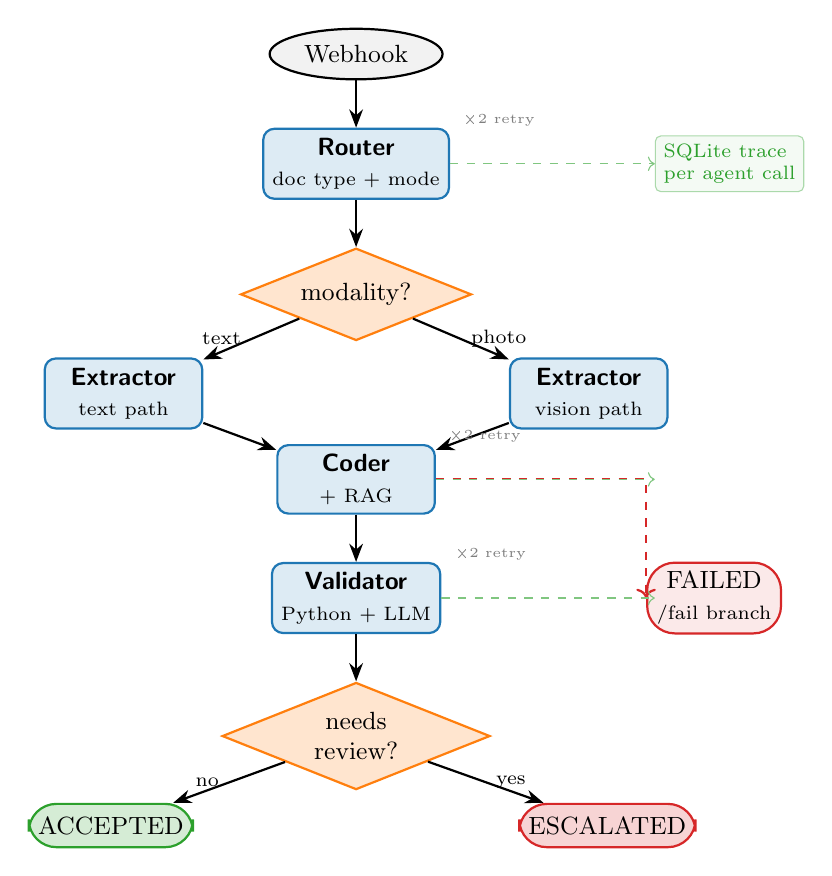
\begin{tikzpicture}[
  every node/.style={font=\small},
  node distance=0.6cm and 1.1cm,
  agent/.style={draw, rounded corners=4pt, minimum width=2.0cm,
                minimum height=0.65cm, thick, fill=C1!15, draw=C1, align=center},
  dec/.style={draw, diamond, minimum width=1.8cm, minimum height=0.65cm,
              thick, fill=C2!20, draw=C2, aspect=2.5, align=center},
  term/.style={draw, rounded corners=10pt, minimum width=1.7cm,
               minimum height=0.55cm, thick, align=center},
  wh/.style={draw, ellipse, fill=gray!10, minimum width=1.4cm,
             minimum height=0.5cm, thick},
  arr/.style={-Stealth, thick},
  lbl/.style={font=\scriptsize, midway},
]
  \node[wh]                    (wh)  {Webhook};
  \node[agent, below=of wh]    (rt)  {\agent{Router}\\{\scriptsize doc type + mode}};
  \node[dec,   below=of rt]    (sw)  {modality?};

  \node[agent, below left=0.5 and 1.2 of sw]  (extT) {\agent{Extractor}\\{\scriptsize text path}};
  \node[agent, below right=0.5 and 1.2 of sw] (extV) {\agent{Extractor}\\{\scriptsize vision path}};

  \node[agent, below=1.3cm of sw] (co)  {\agent{Coder}\\{\scriptsize + RAG}};
  \node[agent, below=of co]       (va)  {\agent{Validator}\\{\scriptsize Python + LLM}};
  \node[dec,   below=of va]       (rv)  {needs\\review?};

  \node[term, below left=0.5 and 1.2 of rv,
        fill=accepted!20, draw=accepted]  (acc) {ACCEPTED};
  \node[term, below right=0.5 and 1.2 of rv,
        fill=escalated!20, draw=escalated](esc) {ESCALATED};

  % right side: fail branch
  \node[term, right=2.6cm of va, fill=C4!10, draw=C4] (fail) {FAILED\\{\scriptsize /fail branch}};

  % arrows main path
  \draw[arr] (wh)  -- (rt);
  \draw[arr] (rt)  -- (sw);
  \draw[arr] (sw)  -- node[lbl, left]{text}  (extT);
  \draw[arr] (sw)  -- node[lbl, right]{photo} (extV);
  \draw[arr] (extT) -- (co);
  \draw[arr] (extV) -- (co);
  \draw[arr] (co)  -- (va);
  \draw[arr] (va)  -- (rv);
  \draw[arr] (rv)  -- node[lbl, left]{no}  (acc);
  \draw[arr] (rv)  -- node[lbl, right]{yes} (esc);

  % fail branch
  \draw[->, dashed, draw=C4, thick]
    (co.east) -- ++(0.5,0) -- (fail.west |- co) -- (fail.west);

  % SQLite note
  \node[right=2.6cm of rt, font=\scriptsize, color=C3, align=left,
        draw=C3!40, rounded corners=2pt, fill=C3!5, inner sep=3pt]
    (db) {SQLite trace\\per agent call};
  \draw[->, dashed, C3!60] (rt.east)  -- ++(0.4,0) -- (db.west |- rt);
  \draw[->, dashed, C3!60] (co.east)  -- ++(0.4,0) -- (db.west |- co);
  \draw[->, dashed, C3!60] (va.east)  -- ++(0.4,0) -- (db.west |- va);

  % retry annotation
  \foreach \n in {rt, co, va}
    \node[above right=-0.1 and 0.05 of \n, font=\tiny, color=C6]{×2 retry};
\end{tikzpicture}
\caption{The n8n processing path. Routing is deterministic; extraction, coding,
validation, and exception handling are separate service stages. Service calls
write traces to SQLite with step, duration, skill version, and retrieved chunks.}
\label{fig:pipeline}
\end{figure*}

\subsection{Design Rationale}

Table~\ref{tab:design} summarises the key choices and the alternatives considered.

\begin{table}[ht]
\caption{Design choices and rationale}
\label{tab:design}
\centering\scriptsize\renewcommand{\arraystretch}{1.25}
\begin{tabularx}{\columnwidth}{@{}lXX@{}}
\toprule
\textbf{Choice} & \textbf{What we use} & \textbf{Why not the alternative} \\
\midrule
Orchestrator & n8n visual workflow & Custom code gives no visual canvas or
                                     built-in retry \\
LLM provider & Kimi-K2.5 via Azure AI Foundry &
               Selected deployment; median Extractor latency was 1.688\,s in a
               10-document synthetic text benchmark \\
Validation logic & Deterministic Python & LLMs hallucinate arithmetic; Python
                                         is exact \\
Account code grounding & RAG over rules file &
               Observed Company A Coder scores: 0.30 with RAG, 0.10 without \\
Skill versioning & \texttt{v001.md}, \texttt{v002.md}, \ldots &
               Hard-coded prompts cannot be updated without code changes \\
Skill optimization & SkillOpt 0.2.0 adapter & The library proposes bounded
                                skill edits; a continuous held-out gate keeps
                                the current version unless a measured gain is
                                achieved \\
\bottomrule
\end{tabularx}
\end{table}

% ============================================================
%  Section 4 — Data
% ============================================================
\section{Synthetic Corpus}
\label{sec:data}

\subsection{Document Generation}

We generate 300 documents (150 per company) using a deterministic Python generator
seeded at 42, so every run produces the identical corpus. Documents are PDFs with
a text layer (ReportLab~\cite{reportlab}) plus a degraded photo variant.
All text is in French.

Each generated document contains a selected set of accounting-style fields:
supplier name, a synthetic matricule fiscal (7 digits + letter), date in
\textit{jj/mm/aaaa} format,
line items with HTVA/TVA/TTC amounts, a Timbre Fiscal line, and the document total.
Amounts use the French format with a narrow no-break space as thousands separator
(e.g., \textit{1\,011,500\,TND}).

\textbf{Company A} uses TND currency, 19\% VAT on all lines, and six-character
account codes such as \textit{606100}.

\textbf{Company B} uses EUR and TND, tiered VAT at 7\%, 13\%, or 19\% per line,
and account codes of the form \textit{6060-EN001}.

Photo variants add synthetic degradation: rotation between 8° and 15°,
Gaussian noise with $\sigma \in [15,20]$, and JPEG quality between 55 and 65.
They are not a substitute for independently collected, real-world scans.

\subsection{Error Injection}

30\% of documents contain exactly one injected error:

\begin{itemize}[leftmargin=*, itemsep=2pt]
  \item \textbf{Arithmetic mismatch}: the TTC printed on the document does not
        equal HTVA + TVA, triggering the Validator's deterministic check.
  \item \textbf{Missing matricule}: the supplier's tax identifier field is blank.
  \item \textbf{Duplicate ID}: the document is marked as a copy of an existing
        one via a \texttt{duplicate\_of} field.
\end{itemize}

Documents with injected errors should exit as \texttt{ESCALATED}; clean documents
should exit as \texttt{ACCEPTED}. This gives us a ground-truth label for measuring
Validator F-score.

\subsection{Hidden House Rules}

Each company has four hidden rules stored separately from the public RAG corpus
and represented in generated gold metadata. Company B's rules cover EUR invoice
conversion, review of high-value TechVision invoices, a fixed AssurPlus code,
and a flag for Station Total purchase orders. The corpus generator also assigns
TechVision consulting and audit line items to \texttt{6226-HO001}; seven such
TRAIN examples support the v003 skill exception evaluated in
\cref{sec:skillopt}. These company policies are synthetic and are not official
Tunisian accounting guidance.

\subsection{Splits and Integrity}

\begin{table}[ht]
\caption{Corpus statistics}
\label{tab:corpus}
\centering\scriptsize\renewcommand{\arraystretch}{1.2}
\begin{tabular}{@{}lrrrr@{}}
\toprule
\textbf{Split} & \textbf{Size} & \textbf{Co.\,A} & \textbf{Co.\,B} & \textbf{Purpose} \\
\midrule
TRAIN     & 140 & 70 & 70 & Skill development \\
SELECTION & 60  & 30 & 30 & Baseline eval, validation \\
TEST      & 100 & 50 & 50 & Final comparison (held-out) \\
\midrule
Total & 300 & 150 & 150 & \\
\bottomrule
\end{tabular}
\end{table}

The SkillOpt pilot used a balanced sample of 12 Company B TRAIN and 12 Company B
SELECTION items from the project data, rather than the full split. It did not
evaluate the TEST partition.

Seven automated integrity checks verify the corpus on every generation:
unique IDs across all 300 documents, no document in more than one split,
arithmetic consistency of all gold labels except injected-error documents,
all account codes present in the company chart, house-rule text absent from
public files, all matricule fiscal values matching the 7-digit+letter pattern,
and no generic placeholder text.

% ============================================================
%  Section 5 — Agents
% ============================================================
\section{Agent Design}
\label{sec:agents}

Each agent loads its system prompt from a versioned Markdown file at
\texttt{skills/<company>/<agent>/vNNN.md}. The loaded version is logged in
SQLite traces, making the prompt used for a decision inspectable. Agents are
independent: updating the Extractor skill does not touch the Coder or Validator.

\subsection{LLM Client}

The LLM-calling stages use a shared \texttt{LLMClient} that wraps Azure AI
Foundry and OpenAI-compatible endpoints; the deterministic Router does not call
an LLM. Provider and model roles are configured through environment variables.
The current client configuration:
\begin{itemize}[leftmargin=*, itemsep=1pt]
  \item Sets temperature to 0 for model calls.
  \item Reads reasoning effort per role from configuration; the reported
        baseline and latency benchmark used \texttt{reasoning\_effort=none}.
  \item Removes returned reasoning content before passing text downstream;
        the client logs an approximate word count when that content is present.
  \item With \texttt{DEMO\_CACHE=1}, responses are cached by a SHA-256 hash
        of the full prompt. Cache hits incur zero network calls — useful for
        reproducible demos.
\end{itemize}

\subsection{Router}

The \agent{Router} determines the document type (\textit{invoice}, \textit{receipt},
\textit{purchase\_order}) and input modality (\textit{text} or \textit{photo}).
In our current implementation it is a deterministic Code node in n8n using file
extension and keyword matching — no LLM call. This avoids a model request but
can misroute files with unfamiliar extensions or ambiguous text; it is not
fail-proof.

\subsection{Extractor}

The \agent{Extractor} converts a document into a structured JSON object with all
fields the Validator and Coder need: supplier, date, document number, each line item
with its amounts, HTVA, TVA, TTC, Timbre Fiscal, and the matricule fiscal.
For text-layer PDFs, text is extracted via \texttt{pypdf}. For photos, the image
is sent to the vision deployment and the model's transcription is treated as the
text input.

The skill prompt uses four techniques:
\begin{enumerate}[leftmargin=*, itemsep=1pt]
  \item \textbf{Role prompting} — ``You are an expert Tunisian accounting clerk.''
  \item \textbf{Structured output schema} — the expected JSON schema is listed
        in the system prompt with field names and types.
  \item \textbf{Format guardrails} — explicit instructions for the TND amount
        format, the matricule fiscal pattern, and the date format.
  \item \textbf{Termination instruction} — ``Respond only with the JSON object,
        no explanatory text.''
\end{enumerate}

\subsection{Coder}

The \agent{Coder} assigns a ledger account code and cites the rule it used. Before
the LLM call, the Coder retrieves the five most relevant rule chunks from Qdrant
(filtered to the current company) and injects them into the system prompt. The
score is binary: 1.0 if the code matches the gold label \emph{and} the cited rule
appears as a substring in the retrieved chunks or skill file; 0.0 otherwise. This
is a mechanical support check. It does not verify that the cited text semantically
justifies the code, so the metric is weaker than a human audit of the rationale.

\begin{figure}[ht]
\centering
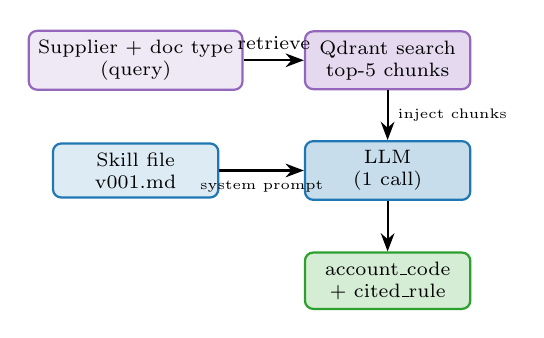
\begin{tikzpicture}[
  every node/.style={font=\scriptsize},
  box/.style={draw, rounded corners=3pt, minimum width=2.1cm,
              minimum height=0.6cm, thick, align=center},
  arr/.style={-Stealth, thick},
]
  \node[box, fill=C5!15, draw=C5]  (q)  at (0,0)    {Supplier + doc type\\(query)};
  \node[box, fill=C5!25, draw=C5]  (qd) at (3.2,0)  {Qdrant search\\top-5 chunks};
  \node[box, fill=C1!15, draw=C1]  (sk) at (0,-1.4) {Skill file\\v001.md};
  \node[box, fill=C1!25, draw=C1]  (lm) at (3.2,-1.4){LLM\\(1 call)};
  \node[box, fill=C3!20, draw=C3]  (out)at (3.2,-2.8){account\_code\\+ cited\_rule};

  \draw[arr] (q)  -- node[above, font=\scriptsize]{retrieve} (qd);
  \draw[arr] (qd) -- node[right, font=\tiny]{inject chunks} (lm);
  \draw[arr] (sk) -- node[below, font=\tiny]{system prompt} (lm);
  \draw[arr] (lm) -- (out);
\end{tikzpicture}
\caption{Coder agent flow: RAG retrieves relevant rules, which are injected
alongside the skill prompt into a single LLM call.}
\label{fig:coder_flow}
\end{figure}

\subsection{Validator}

The \agent{Validator} runs in two phases. First, three deterministic Python checks
run without any LLM call:
\begin{itemize}[leftmargin=*, itemsep=1pt]
  \item Arithmetic: $|\text{HTVA} + \text{TVA} - \text{TTC}| \leq 0.005$ currency units.
  \item Matricule fiscal present and non-empty.
  \item A duplicate marker check if \texttt{duplicate\_of} is present in the extracted payload.
\end{itemize}
If any check fails, a single LLM call generates a one-sentence explanation for
the human reviewer, and \texttt{needs\_review} is set to \texttt{true}.

Alongside the supplied \texttt{duplicate\_of} marker, the API registers a
normalized company, supplier, invoice-number, and date key in SQLite; a match
identifies the earlier document and routes the new item for review. Replays of
the same document ID are idempotent. Keeping validation logic in Python rather than delegating it to the LLM is a
deliberate choice: arithmetic at a 0.005 currency-unit tolerance is computed in Python and
unreliable in an LLM, especially for Tunisian formatting with three decimal places.

\subsection{Exception Handler}

When the Validator raises a flag, the \agent{Exception Handler} prepares a
structured escalation dossier: a summary of the errors, the recommended action
(correct the arithmetic / re-request the document / contact the supplier), and
the responsible contact. This is stored as a JSON object in SQLite for later
review; the current workflow does not send an external notification to a reviewer.

% ============================================================
%  Section 6 — RAG Engine
% ============================================================
\section{RAG Engine}
\label{sec:rag}

\subsection{Retrieval Design}

The Coder uses retrieval to ground account assignment in a company's own
accounting rules. The local knowledge base contains a chart of accounts and
topic-level Markdown policy sources per company. Inference embeds a query built
from supplier, document type, and description; Qdrant returns up to five chunks
filtered by \texttt{company\_id}. Retrieved text is passed alongside the
company's versioned Coder skill. The embedding model is
\texttt{paraphrase-multilingual-mpnet-base-v2} (768 dimensions), and the vector
store runs locally in embedded mode.

The implementation supports two chunkers. The default fixed-window strategy
uses 512 tokens with a 64-token overlap. The heading-based strategy groups
Markdown sections up to 1024 tokens. These choices are recorded for comparison;
the present corpus is too small to establish a winning strategy.

\subsection{What the Retrieval Evaluation Establishes}

Twenty hand-written queries per company were evaluated against expected policy
source filenames. With fixed chunks, source-level Recall@5 is 1.00 for both
companies; MRR@5 is 0.9167 for Company A and 0.8875 for Company B. With heading
based chunks, Recall@5 remains 1.00; MRR@5 is 0.9167 and 0.8500, respectively.
The fixed corpus contains 9 Company A chunks and 11 Company B chunks; the
heading corpus contains 9 and 10.

These figures should not be read as rule-level retrieval accuracy. The corpus
is still small relative to top-k=5, and the label only checks whether the
expected policy source appears; it does not identify the correct rule within
that source. Recall@5 is therefore saturated, and this small comparison does
not support a chunking winner. The evaluation verifies that company-filtered
retrieval returns the expected source, but it does not show that the best rule
ranks first or that retrieval improves accounting decisions.

The coding ablation in \cref{tab:baseline_main} is separate evidence: on the
reported selection runs, Coder score with retrieval was 0.30 for Company A and
0.21 for Company B, versus 0.10 and 0.00 without retrieval. These are low
absolute scores on synthetic data and do not isolate retrieval quality from
model and prompt errors. A stronger next evaluation should split the knowledge
base into individual rule chunks, label relevant rule IDs for each query, and
report Recall@k, MRR, and per-query examples on a larger rule set.

% ============================================================
%  Section 7 — Evaluation
% ============================================================
\section{Evaluation}
\label{sec:evaluation}

The agent baseline comes from pipeline runs on the SELECTION set (30 synthetic
documents per company, 60 total) using skill version v001. Vision and latency
figures come from separate, smaller synthetic benchmarks. They describe these
fixtures and should not be interpreted as production performance.

\subsection{Metrics}

\textbf{Extractor NEM} (Normalized Exact Match): fraction of gold fields for
which the predicted value, after stripping whitespace, lowercasing, and converting
French number format to decimal, exactly matches the gold label.

\textbf{Coder Score}: binary — 1.0 only if the account code matches the gold
label and the cited string appears in a retrieved chunk or skill file. This is a
substring check; it does not establish that the citation semantically supports
the decision.

\textbf{Validator F-$\beta$} ($\beta\!=\!\sqrt{2}$): a weighted F-score where
missing an error (false negative) costs twice as much as a false alarm (false
positive). This reflects the accounting domain: an undetected arithmetic error
is worse than an unnecessary escalation.

\textbf{Vision accuracy}: fraction of key fields (supplier, document number, TTC)
correctly read from synthetic degraded images, measured on 12 generated
documents.

\subsection{LLM Health Check}

Before running any agents, a doctor script validates the model:

\begin{table}[ht]
\caption{LLM health check results (Kimi-K2.5, \texttt{reasoning\_effort=none})}
\label{tab:doctor}
\centering\scriptsize\renewcommand{\arraystretch}{1.2}
\begin{tabular}{@{}lcc@{}}
\toprule
\textbf{Check} & \textbf{Result} & \textbf{Pass?} \\
\midrule
Vision accuracy — supplier (N=12)    & 12/12 = 100\% & \checkmark \\
Vision accuracy — TTC (N=12)         & 12/12 = 100\% & \checkmark \\
Reasoning tokens in agent calls      & 0             & \checkmark \\
Extractor median latency (N=10)      & 1{,}688\,ms   & \checkmark \\
Extractor p95 latency                & 2{,}765\,ms   & \checkmark \\
JSON parse rate (text docs, N=10)    & 10/10 = 100\% & \checkmark \\
\bottomrule
\end{tabular}
\end{table}

In this sample, the vision model read the three reported fields correctly on all
12 generated images, and the text benchmark parsed JSON on all 10 documents.
These small, synthetic checks do not establish general image or extraction
accuracy. The 1.688\,s median is Extractor latency only; end-to-end latency was
not measured in this benchmark.

\subsection{Baseline Results}

\begin{table}[ht]
\caption{Baseline scores on SELECTION set, skill v001 (real runs)}
\label{tab:baseline_main}
\centering\scriptsize\renewcommand{\arraystretch}{1.25}
\begin{tabular}{@{}lrrr@{}}
\toprule
\textbf{Company} & \textbf{Coder+RAG}
                 & \textbf{Coder\,\,noRAG} & \textbf{Val.\,$F_\beta$} \\
\midrule
Company A (N=30) & 0.300 & 0.100 & 0.108 \\
Company B (N=30) & 0.205 & 0.000 & 0.000 \\
\midrule
Macro average    & 0.253 & 0.050 & 0.054 \\
\bottomrule
\end{tabular}
\end{table}

The earlier Extractor NEM values are omitted. The baseline scorer treated
unsupported or mis-mapped fields as errors; the corrected scorer is available,
but the full baseline has not been rerun, so no corrected aggregate is claimed.

\begin{figure}[ht]
\centering
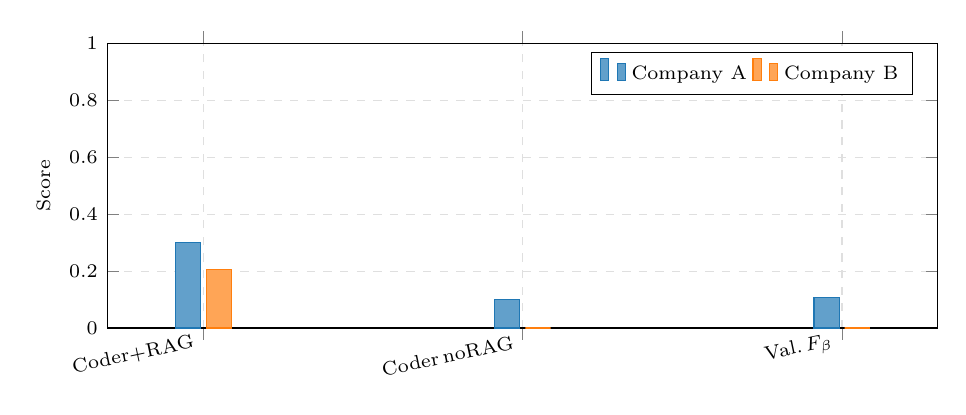
\begin{tikzpicture}
\begin{axis}[
  width=\columnwidth, height=5.2cm,
  ybar, bar width=0.32cm,
  ymin=0, ymax=1.0,
  ylabel={Score},
  ylabel style={font=\scriptsize},
  symbolic x coords={Coder+RAG, Coder\,noRAG, Val.\,$F_\beta$},
  xtick=data,
  x tick label style={font=\scriptsize, rotate=12, anchor=east},
  tick label style={font=\scriptsize},
  legend style={font=\scriptsize, at={(0.97,0.97)}, anchor=north east,
                legend columns=2},
  grid=major, grid style={dashed, gray!25},
  enlarge x limits=0.15,
]
\addplot[fill=C1!70, draw=C1]   coordinates {
  (Coder+RAG,0.300)(Coder\,noRAG,0.100)(Val.\,$F_\beta$,0.108)};
\addplot[fill=C2!70, draw=C2]   coordinates {
  (Coder+RAG,0.205)(Coder\,noRAG,0.000)(Val.\,$F_\beta$,0.000)};
\legend{Company A, Company B}
\end{axis}
\end{tikzpicture}
\caption{Baseline agent scores per company on the SELECTION set (skill v001,
real pipeline runs). The with/without-RAG comparison is a small observational
ablation, not a general causal estimate.}
\label{fig:baseline_bars}
\end{figure}

\subsection{What the Numbers Mean}

\textbf{Extractor.} The previously reported 0.61 / 0.31 values are withdrawn.
The baseline scorer counted a benchmark-only reference field and failed to map
line descriptions from the production nested schema. The evaluation needs to be
rerun with the corrected scorer before an Extractor baseline can be reported.

\textbf{Coder 0.30 / 0.21 with RAG.}
These are low scores from earlier full-pipeline runs. A new paired prompt
comparison isolated Company B coding with gold extracted fields and identical
top-5 RAG context on 10 fixed SELECTION documents. Code accuracy rose from
7/10 to 9/10; the stricter correct-code-plus-supported-citation score rose
from 2/10 to 6/10. The improved prompt won four cases, lost none, and tied six.
This small selection sample is promising but is neither a full-corpus nor a
held-out TEST result. The older v001/v002 comparison remains rate-limited and
inconclusive. See \cref{sec:skillopt} and
\url{eval/results/company_b_coder_improvement.json}.

\textbf{Validator F-$\beta$ 0.11 / 0.00.}
These low scores show that validation and the baseline evaluator need further
work. We do not claim that a later code change improved them because no
comparable rerun is available. A useful next experiment should report
per-check precision and recall as well as the aggregate F-score.

The reported retrieval figures are source-level and saturated because each
company has only two or three chunks. See \cref{sec:rag} for the metric limits.

% ============================================================
%  Section 8 — Skill optimization and measured prompt iteration
% ============================================================
\section{Company-Specific Skill Adaptation}
\label{sec:skillopt}

\subsection{SkillOpt Integration and Evaluation}

DocDesk represents company behaviour as versioned Markdown skills. The actual
SkillOpt 0.2.0 library runs against the Extractor environment through the
product API. It receives labeled TRAIN examples, groups failure feedback into
bounded skill patches, then evaluates candidate changes on a disjoint SELECTION
split. A candidate is promoted only when the configured continuous score
improves. Model weights are unchanged; TEST remains reserved for a final
comparison.

The Company B run used 12 TRAIN, 20 SELECTION, and 10 TEST documents, covering
invoices, purchase orders, and receipts. The dataset snapshots and SHA-256
hashes are saved with the run. Kimi-K2.5 served both the target and optimizer
roles. The initial skill scored 1.00 hard exact match on SELECTION. Across
three four-example TRAIN steps, SkillOpt skipped all edits because selection
performance did not improve; the initial skill remained the best version. The
run took 1,041.5 seconds and recorded 97,805 tokens across 37 calls. These
values are specific to this small generated pilot, not a general-purpose
accuracy estimate.

The first baseline TEST pass returned exact scores for 4 of 10 documents; six
were lost to temporary provider connection errors. Retrying those six produced
valid exact predictions for all six. A fresh run of the selected skill also
completed all 10 documents with exact predictions. Thus both the recovered
baseline and selected skill scored 10/10 exact on this held-out set, while the
selected skill is byte-identical to the initial skill. This is evidence of no
measured change, not an optimization gain. Retry-aware counts and per-document
records are in \url{eval/results/company_b_extractor_skillopt.json}; raw
outputs and dataset fingerprints are preserved under
\url{skillopt_output/company_b_extractor/runs/20261019T155925Z}.

The previously reported broad Extractor NEM is not comparable: its scorer
counted \texttt{reference\_unique}, which the production response schema does
not return, and failed to map gold \texttt{line\_descriptions} to nested
production \texttt{lines[].description}. Both mismatches guaranteed field
errors. The scorer is corrected in the repository, but the broad baseline has
not been rerun; its old Extractor NEM values are withdrawn. The SkillOpt pilot's
1.00 selection score uses the corrected field mapping on only 20 SELECTION items,
so it remains an adapter-level result rather than a broad production accuracy
claim. The optimizer made no skill change and provides no evidence of an
accuracy gain.

To make the adaptation mechanism visible, a separate demo-only run started from
an intentionally poor prompt that always returned \texttt{UNKNOWN}. On 20
SELECTION documents, its soft normalized exact-match score rose from 0.01 to
0.21 after SkillOpt accepted bounded edits. Hard exact match remained 0.00 for
both prompts. On the untouched 10-document TEST split, soft NEM rose from 0.02
to 0.17, but hard exact match remained 0/10 for both. This shows improved
partial-field overlap, not successful complete extraction. The weak prompt is
isolated from the production skill and is included only to demonstrate the
optimizer. Artifacts are stored under
\url{skillopt_output/company_b_extractor_showcase}.

\subsection{Separate Manual Prompt Iteration}

We used the existing Company B TRAIN labels to investigate a measured
Coder error. Seven training documents showed that TechVision consulting,
audit, and research work maps to \texttt{6226-HO001}, while technical IT work
maps to \texttt{6170-IT001}. The v003 prompt added this exception. The broader
v004 revision added an explicit supplier-to-account map, made supplier identity
the primary signal for this benchmark, preserved line-description
disambiguation for TechVision's mixed services, and required short verbatim
citations.

\begin{table}[ht]
\caption{Company B Coder prompt comparison on the SELECTION split}
\label{tab:skill_iteration}
\centering\scriptsize\renewcommand{\arraystretch}{1.2}
\begin{tabular}{@{}lrrr@{}}
\toprule
\textbf{Metric} & \textbf{Baseline v001} & \textbf{Improved v004} & \textbf{Change} \\
\midrule
Cases (paired SELECTION) & 10 & 10 & -- \\
JSON parse rate & 10/10 & 10/10 & 0 \\
Correct account code & 7/10 & 9/10 & +2 \\
Supported code and citation & 2/10 & 6/10 & +4 \\
\bottomrule
\end{tabular}
\end{table}

Both prompts received the same gold extracted fields and identical
company-filtered top-5 RAG results, isolating the coding skill from OCR and
extraction quality. On the paired sample, v004 improved code accuracy by 20
percentage points and the stricter supported score by 40 points; it won four
cases, lost none, and tied six. All 10 responses parsed. This remains a small
selection-only prompt experiment, not a full-corpus or held-out TEST estimate.
The earlier four-case TechVision comparison remains a development check. Full
per-document outputs are in
\url{eval/results/company_b_coder_improvement.json}; prompt text and notes are
in \texttt{prompts/PROMPT\_LIBRARY.md}.

A separate 30-document v001/v002 run was throttled by provider rate limits. Only
12 documents had valid responses from both prompts; their supported Coder
scores were 9/12 and 8/12, respectively. This incomplete run is not evidence
that v002 improved performance. It motivated bounded requests, checkpointing,
and explicit separation of provider errors from model errors in the evaluator.

\subsection{Interpretation}

The v004 result is a manual, train-informed prompt revision; it is separate
from SkillOpt and must not be described as optimizer-generated. It is early
paired evidence from 10 SELECTION examples. The production skill loader selects
v004; TEST evaluation remains necessary before claiming generalization. The
older targeted comparison is available in
\texttt{eval/results/company\_b\_skill\_adaptation.json}.

% ============================================================
%  Section 9 — Limitations and next experiments
% ============================================================
\section{Limitations and Next Experiments}
\label{sec:roadmap}

The project is a course prototype with useful evidence and important gaps. We
prioritize the work by the evidence needed to make the company-adaptation claim
reproducible.

\begin{enumerate}[leftmargin=*, itemsep=3pt]
  \item \textbf{Broaden SkillOpt evaluation.} The real library now runs through
        the product API on balanced Company B TRAIN and SELECTION cohorts. The
        next experiment should use the full held-out set, repeat with multiple
        seeds, preserve all candidate traces, and evaluate a selected skill
        once on TEST before claiming a company-wide gain.
  \item \textbf{Confirm the targeted coding result.} Evaluate v003 on the full
        Company B SELECTION and held-out TEST sets, with model calls paced to
        stay within provider limits. Include code accuracy, citation support,
        JSON parse rate, provider errors, and paired uncertainty.
  \item \textbf{Strengthen retrieval evaluation.} The current rule corpus has
        only a few chunks per company, making Recall@5 saturated. Re-chunk at
        rule level, compare fixed and heading-based strategies on the same
        queries and vector model, and report per-query results.
  \item \textbf{Improve task quality.} Expand the synthetic corpus, audit
        company-rule and gold-label consistency, and add independently labeled
        real scans before making real-world accuracy claims. Keep arithmetic
        validation deterministic and report error-type precision and recall.
  \item \textbf{Harden deployment.} Add authentication, role-based review,
        secret management, backups, retention controls, and monitoring before
        using real company financial documents.
\end{enumerate}

No post-baseline score projections are reported. The next release should be
judged by repeatable held-out measurements rather than a target inferred from
unrelated benchmarks.

% ============================================================
%  Security and deployment boundaries
% ============================================================
\section{Security Considerations}
\label{sec:security}

The prototype uses synthetic documents and fictional company policies; no
customer records are included in the evaluation. Provider credentials are read
from environment configuration rather than embedded in prompts or source
control. Retrieval requests include a company filter, and stored decisions
retain a trace of the skill version and evidence used. Validation exceptions
are routed for human review instead of silently treated as approved entries.

These controls are prototype safeguards, not a production security assessment.
Before connecting real mailboxes or Drive folders, an operator must configure
Google OAuth with the minimum required scopes, restrict access to the n8n and
dashboard interfaces, and define retention, backup, deletion, and audit
procedures. Prompts and retrieved document text are untrusted input; the
current prototype does not provide a dedicated prompt-injection defense.
Accounting rules also require review by a qualified professional. Gmail and
Drive triggers remain disabled until credentials and a monitored folder are
configured.

% ============================================================
%  Section 11 — Conclusion
% ============================================================
\section{Conclusion}
\label{sec:conclusion}

DocDesk is a company-adaptive accounting automation prototype built around an
n8n workflow, specialized agents, company-filtered RAG, multimodal document
intake, deterministic validation, human review, and an SQLite audit ledger. Its
central design choice is to keep company-specific accounting behavior in
versioned skills so that changes can be inspected and measured without
fine-tuning model weights.

The existing end-to-end baseline shows higher observed Coder scores with RAG for both
companies, although absolute scores are low and the small rule corpus weakens
the retrieval evaluation. A paired Company B prompt comparison on ten SELECTION
documents raised code accuracy from 7/10 to 9/10 and supported code-plus-citation
from 2/10 to 6/10. It used gold extracted fields and identical RAG, so it
isolates Coder behavior rather than end-to-end processing; the result remains
small-sample selection evidence. The integrated SkillOpt
run processed balanced 12-document TRAIN and SELECTION samples. Initial
extraction scored 1.00 on both in its adapter, despite the broader Company B
Extractor baseline of 0.31. This discrepancy remains unresolved and the two
figures are not directly comparable. All three failure-only steps found no
patches; the optimizer made no edit and produced no accuracy improvement.

The main engineering result is a working multi-stage prototype with measurable
baseline behavior, a narrowly scoped manual prompt comparison, and an integrated
SkillOpt loop. A separate deliberately weak-prompt showcase improved soft NEM
from 0.02 to 0.17 on ten held-out documents, but exact match remained 0/10 for
both versions; this is partial-field progress, not reliable extraction. Before operational use, the
project needs comparable end-to-end evaluation, a larger rule-level retrieval
test, audited business rules, and production security controls.

\section*{Acknowledgments}
This work uses n8n, Qdrant, sentence-transformers, SkillOpt, and synthetic
French-language accounting documents. The charts of accounts are fictional
and must not be treated as verified Tunisian accounting advice.


% --- References ---------------------------------------------
\bibliographystyle{IEEEtran}
\bibliography{references}

% --- Prompt library annex (excluded from the eight-page report limit) ---
\appendices
\section{Prompt Library}
The project prompt versions, techniques, and evaluation evidence are included
below. Complete operational prompts are versioned in the linked repository
files listed in the library.
\lstinputlisting[breaklines=true,basicstyle=\ttfamily\scriptsize]{../prompts/PROMPT_LIBRARY.md}

\end{document}
